\section{Methods}

\subsection{Data}
%\subsubsection{Source}
The \texttt{PISCES Cull PDB} database server (Wang \& Dunbrack, 2003) is a commonly used source for data for evaluating 
machine learning models trained to predict amino secondary structures. Following in the footsteps of the Zhou \& 
Troyanskaya, we have used the same data set as in their 2014 paper \textit{Deep Supervised and Convolutional Generative 
Stochastic Network}, which is a dataset produced by the PISCES server.

The database contains information on 5926 proteins. Zhou \& Troyanskaya have filtered the data such that it contains no proteins consisting of less than 50 or more than 700 amino acids, and have thus encoded each protein as a section of 700 amino acids, the non-existant ones (in the case of a protein of less than 700 amino acids) being marked as \texttt{not sequenced}.

\subsubsection{Features}
Each amino acid in the database contains 57 features (or channels) of information. The first 22 features encode which of the 20 amino acids that occur in genetic code, plus amino acid 'X' representing 'Unknown' as well as 'NoSeq'.

This information is encoded in a one-hot format, meaning that instead of encoding the actual amino acid or the number of the acid, one encodes an array of zeros with only the element at the index of the number of the amino acid being set to one. So in order to encode Glutamic acid (E) i.e. the third amino acid, the one-hotted data would be $[0, 0, 1, 0, 0, ... , 0, 0]$. 

Encoding the data in this way makes very good sence in regard to training classifiers, as if one was to encode amino acid E simply as the number 3 (E being the third amino acid), the classifier would falsely train on the premise that a guess of 4 was a less bad guess than a guess of 15, based on the proximity of the indexes.

The secondary structure labels that the model attempts to predict is encoded in the same manner, however for training purposes we have collapsed it into indexes in our model. Further, as explained above, there are three main forms of protein secondary structures ($\alpha$-helix, $3_{10}$-helix and $\pi$-helix), however within them there are further 8 sub-forms of structures, which are the ones that are encoded in the dataset.

\end{multicols}
\begin{table}[h]
\centering
\begin{tabular}{l|l|l}
Feature nr.   & Feature                                     & Encoding                 \\ \hline
{[} 0,22{[}   & Amino acid residues                         & One-hot                  \\
{[}22,31{[}   & Secondary structure labels                  & One-hot                  \\
{[}31,33{[}   & N- and C-terminals                          & Binary                   \\
{[}33,35{[}   & Relative and absolute solvent accessibility & Binary                   \\
{[}35,57{[}   & Sequence profile                            & Probability distribution
\end{tabular}
\end{table}
\newpage
\begin{multicols}{2}
\noindent The N- and C-terminals indicate whether the amino acid in question is the first or the last in the protein chain and are encoded binarily.

While the solvent accessibility features in the PISCES database are encoded as floating point numbers, the creators of the dataset in question have followed the practice of (Qi et. al., 2012) and discretizised the values to binary values. The threshold for absolute accessibility is 15, while relative accessibility is "is normalized by the largest accessibility value in a protein and thresholded at 0.15" (Zhou \& Troyanksaya, 2014).

The sequence profile in the final 22 features is calculated using the \textit{Position-Specific Scoring Matrix} (PSSM) system, and is used to indicate that if it had not been the amino acid in question that was present at this specific position, with what probability would it then statistically have been which of the other amino acids. Interestingly, the order of the amino acids in the sequence profile differs from that of the amino acid residues, however this should not have any impact on the model.


\subsubsection{Splitting the data}
When training our model, we split the above data into three sets: training, validation and test. The purpose of splitting the training data from the evaluation data is to counter possible overfitting, that is, training a model to an extent where it correctly predicts the kinks and quirks of the training set that do not express general tendencies in the system.

The point in further splitting into both a validation and a test set is that we continuously evaluate the loss and accuracy on the validation set (instead of the training set) in order to make decision regarding the architecture and configuration of the model, but to prevent us from humanly overfitting to this set, the test set is held in reserve and is only evaluated once, in the end of a model's training.

In this case, we followed the advice from the documentation accompanying the dataset and split the data into 5430 proteins for training, 255 proteins for testing and 236 proteins for validation. The training set was then further shuffled between each epoch.

In evaluating the optimal hyperparameters for hte model we iterated over different batch-sizes for training (results below).

\subsection{Tools}
\subsubsection{Model}
Being that we are training a convolutional neural network, in particular two sets of functions are important, namely activation and loss functions.

The activation functions we opted to use in this project were the rectifier, softmax and sigmoid functions respectively, whereas we use the Cross Entropy loss in evaluating and training the network.
\paragraph{Rectifier}
Possibly the simplest of these activation functions is the rectifier, which when implemented in an artificial neural network is referred to as a \textit{rectified linear unit} (ReLU), which, in laymans terms, simply does not allow negative values, and replaces such values with zero.
\[
ReLU(x) = x^+ = max(0,x)
\]

\paragraph{Sigmoid function}
Sigmoid functions are a specific variant of logistic functions, and serve to map values in arbitrary ranges to values within a specific range, so that the mapped values over the original values form a sigmoid curve. The value of applying sigmoid functions to outputs from a neural network is that they then enable the model to map its output of arbitrarily big or small values to a probability (i.e. a value $0\leq x \leq 1$). In the present case, this becomes relevant when predicting relative and absolute solvent accessibilities.
\[
Sigmoid(x) = \frac{1}{1 + e^{-x}} = \frac{e^x}{e^x +1}
\]

\begin{Figure}
 \centering
 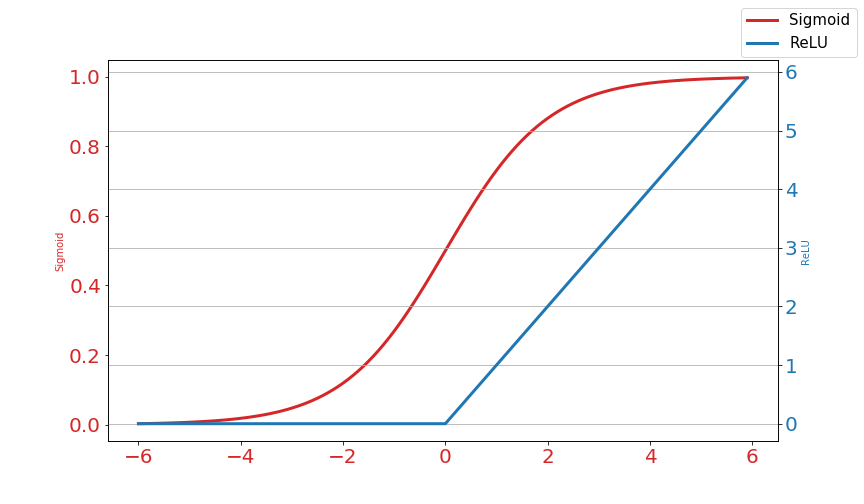
\includegraphics[width=\linewidth]{../graphs/activation.png}
 \captionsetup{width=0.8\linewidth, font=small}
 \captionof{figure}{The sigmoid and rectifier activation functions}
\end{Figure}

%\begin{wrapfigure}{I}{\linewidth}
%\centering
%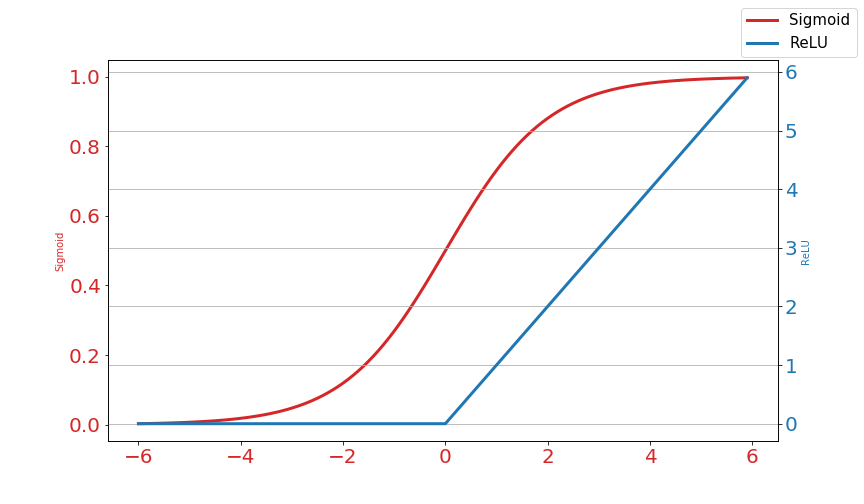
\includegraphics[width=\linewidth]{../graphs/activation.png}
%\caption{This is the former Share\LaTeX{} logo}
%\end{wrapfigure}

%\begin{figure}[h]
%  \centering
%  \frame{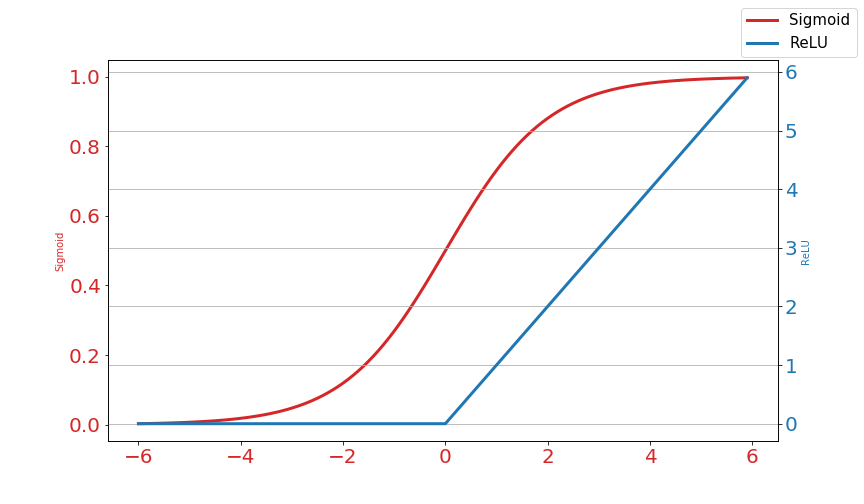
\includegraphics[width=\textwidth]{../graphs/activation}}
%  \caption{The sigmoid and rectifier activation functions}
%\end{figure}

\paragraph{Softmax}
The softmax function ($\sigma$) does very much the same as the sigmoid, only for a range of values. In other words, a set of non-normalized values (that is: of arbitrary length and spread) can via softmax be mapped to a probability distribution over that set. This means that all the values $x_i$ are in the range $0\leq x_i \leq 1$, and that they sum to 1.

This is especially relevant in cases where one is attempting to perform classification, such as which is the present case where we are training the model to predict amino acid secondary structures. 

Applying a softmax function on a dataset \textit{x} of \textit{j} elements would be as follows:
$$
\sigma(x_i) = \frac{e^{x_i}}{\sum_{j=1} e^{x_j}}
$$

\begin{Figure}
 \centering
 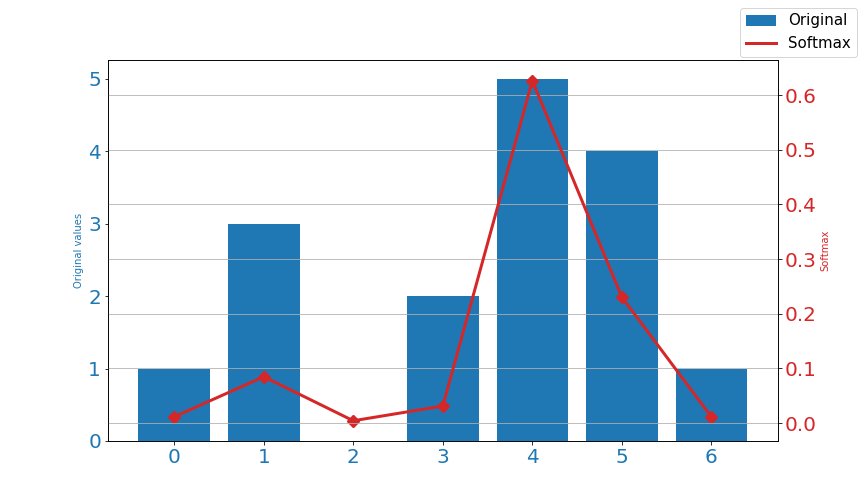
\includegraphics[width=\linewidth]{../graphs/softmax}
 \captionsetup{width=0.8\linewidth, font=small}
 \captionof{figure}{Example data softmaxed}
\end{Figure}
One will often see a very similar function called the \textit{Logarithmic Softmax} which resembles the above, but with the addition that the probability $\sigma(x_i)$ equals the natural logarithm of the same:
\[
\sigma_{log}\left(x_{i}\right)=\log \left(\frac{e^{ x_{i}}}{\sum_{j=1} e^{ x_{j}}}\right)
\]
In practical implementations this approach helps preventing possible underflows.

%\begin{figure}[h]
%  \centering
%  \frame{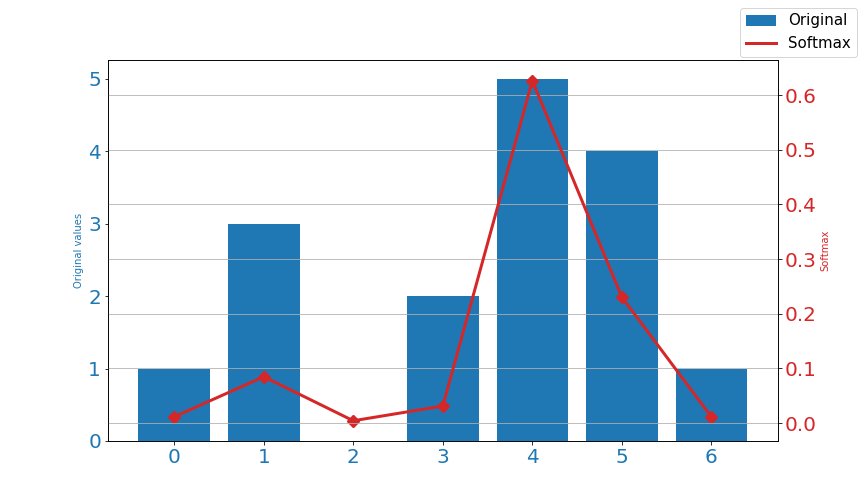
\includegraphics[width=\linewidth]{../graphs/softmax}}
%  \caption{Example data softmaxed}
%\end{figure}


\paragraph{Cross Entropy Loss}
Between two probability distributions each over the same set of outcomes there exists a certain cross entropy.
Thus, given two probability distributions \textit{m} and \textit{n} predicting the discrete outcome $\mathcal{Z}$, the formula for calculating the cross entropy is:
$$L ( m , n ) = - \sum _ { z \in \mathcal { Z } } m ( z ) \log n ( z )$$
A specific instance of the cross entropy loss is the \textit{binary cross entropy loss}, which is useful in cases where the possible outcome is binary (i.e. there are only two possible outcomes). 
\\
Seing as the aim of this paper was to train our network to perform classifications first on amino acid secondary structures (of which there are eight) and then relative and absolute solvent accessibility (which are both encoded as either ones or zeros), we have used a Cross Entropy Loss function on the former and a Binary Cross Entropy Loss function on the two latter.


\subsubsection{Technological implementation details}
In training our network we utilized a machine learning framework for Python called \href{https://pytorch.org/}{PyTorch}, specifically optimized for building deep neural networks. \\
The PyTorch library is build upon the \href{http://torch.ch/}{Torch} library, originally a machine learning library and language based on the scripting language Lua.\\
The strength in using PyTorch stems from several aspects:
\paragraph{GPU support}
PyTorch provides a strong framework for performing calculations on a graphical processing unit rather than the computer's CPU. While GPUs are valued in video game circles, they are also enourmously useful for performing machine learning, since this is often tasks that involve a high number of calculations that can perfectly fine be performed in parallel. For this, a GPU is preferred over a CPU since they often have a much higher number of cores, and are thus better suited for parallel programming. Indeed in our case, there was a factor of 20 difference in the time needed to train an epoch between doing it on the CPU versus the GPU.
\paragraph{Tensors}
The main data structure used in the PyTorch framework is tensors. Where a vector is a 1-dimensional array and a matrix a 2-dimensional array, a tensor is a multi-dimensional array. This means they can be 1-, 2-, 3- or even 42-dimensional arrays. As such tensors subsume scalars, vectors and matrices. (KILDE ER DEEPLEARNING BOGEN p 211). Tensors in PyTorch are multi-dimensional arrays much like the ones implemented in numpy, but with the option to place it on the GPU rather than the CPU.

\paragraph{Automatic differentiation}
In order to utilize the backpropagation that lets neural networks train and improve, the loss must be differentiated in regards to all of the weights and values in the model in order to calculate the gradients. This can be a cumbersome task when performed by hand, but PyTorch provides a powerful tool in for of the \texttt{autograd} and \texttt{optim} modules. The first of these modules keeps track of which computations were performed on which variables in order to arrive at the final value of a variable, so that it can be retraced backwards in the end to calculate gradients, while the latter automatically adjusts the weights and values in the model, according to the calculated gradient and a supplied learning rate.

These things combined indeed allow a training step for a neural network to be performed in as few steps as shown below:
\begin{lstlisting}
# Setup
LR = 0.0025              # learning rate
optimizer = torch.optim.Adam(cnn.parameters(), lr=LR)
loss_func = nn.CrossEntropyLoss()

# One training step
output = cnn(b_x)
loss = loss_func(output, b_y)
optimizer.zero_grad()
loss.backward()
optimizer.step()
\end{lstlisting}

\paragraph{Ready-made implementations}
A final helpful aspect of using PyTorch for implementing artificial neural networks is the abundance of already implemented algorithms and functions. This adds the further detail to the implementation that several of the most often used functions have been written together for reasons of numerical stability. 

For example, the above mentioned Cross Entropy Loss function, which when implemented in PyTorch also contains an implementation of the \texttt{LogSoftmax()} function. The documentation for PyTorch reveals that the implementation then becomes:

\begin{align*}
\operatorname{loss}(x, \text {class})&=-\log \left(\frac{e^{ x[\text {class}]}}{\sum_{j} e^{ x[j]}}\right)\\
&=-x[\text {class}]+\log \left(\sum_{j} e^{x[j]}\right)
\end{align*}

\noindent A similar circumstance is that of the Binary Cross Entropy loss, where PyTorch provides an implementation in the form of \texttt{BCEWithLogitsLoss()} which readily combines the Binary Cross Entropy Loss with a sigmoid function, again in order to provide numerical stability. In this case the implementation becomes: \\
\[
\ell(m, n)=L=\left\{l_{1}, \ldots, l_{N}\right\}^{\top}
\]
where
\[ \quad l_{n}=-w_{n}\left[n_{n} \cdot \log m_{n}+\left(1-n_{n}\right) \cdot \log \left(1-m_{n}\right)\right]
\]

\subsubsection{Hardware}
In terms of performing the calculations, all of our training of the model was done on a Dell PC with a 7th gen octocore Intel Core i7 CPU, 16GB of RAM and a Nvidia GeForce GTX 1050TI GPU with 4GB of RAM and 768 cores running Linux.

\subsection{Single-task secondary structure prediction}
We built a convolutional neural network, implemented in Python using PyTorch in order to predict amino acid secondary structures from the amino acid residues as well as the sequence profile. We tested variations on number of layers, layer depth, kernel sizes and learning rate (results below) in order to maximize performance of the model. 

\subsubsection{Architecture}

The basic structure of the model remained unchanged throughout these test. The basics of the structure was comprised of following elements:
\begin{itemize}
\item It was to be a deep neural network (i.e. at least one hidden layer of neurons),
\item The layer debth was to remain the same throughout the network,
\item Sufficient padding was to be added to the convolving layers so that the breadth of the intermediary values remained the same (the 700 amino acids, that is),
\item After each layer, save the last, the layer was activated using a rectified linear unit,
\item The model should not itself contain a SoftMaxing layer, since this was built into the loss function,
\item The model was evaluated and optimized based on the output of a Cross Entropy loss function,
\item The model was to be optimized based on the loss on the training set while being continuously humanly evaluated on the loss and accuracy on the validation set.
\end{itemize}

\begin{Figure}
 \centering
 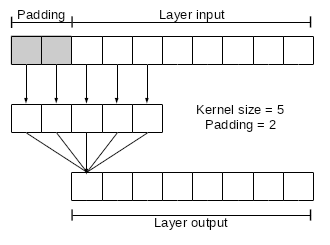
\includegraphics[width=\linewidth]{../graphs/padding}
 \captionsetup{width=0.8\linewidth, font=small}
 \captionof{figure}{The layer breadth is preserved across convolutions thanks to padding.}
\end{Figure}

\subsubsection{Accuracy}
Having built a network that was training and improving on the training set data, it was also relevant evaluate the accuracy of the predictions of the network in addition to the calculation of loss on the validation set.

Several approaches to evaluating predictions exist. The output of our model was something of a proxy to a probability distribution, however not a true probability distribution since the model itself did not perform a SoftMax on the output. This was however not an issue, since the index of the largest value in a set of values remains the same before and after being SoftMaxed, and we could thus safely treat the index of the largest value in the un-SoftMaxed output as the label of the prediction.

In implementing a procedure to evaluate the accuracy of a prediction, we first collapse the output distribution as just described, and then produce a matrix of indicators as to whether the predicted label matched the label in the matrix of actual secondary structure labels as provided by the database.

Of course at this point the model would also be evaluated on its accurate prediction of padding (a task that proved remarkably managable), and thus could achieve arbitrarily high accuracy just by adding more padding to the set. To avoid this, we construct a masking matrix from the values in the target set that are \texttt{NoSeq}. We can then use this mask to filter out the irrelevant values in our matrix of correct and false predictions.

Finally taking the mean of this, now filtered, matrix of prediction correctness produces the percentage of the relevant predictions that were in fact correct.
\begin{Figure}
 \centering
 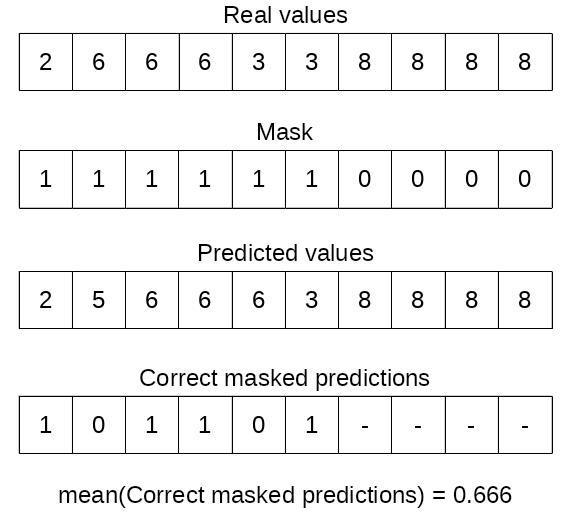
\includegraphics[width=0.8\linewidth]{../graphs/accuracy}
 \captionsetup{width=0.8\linewidth, font=small}
 \captionof{figure}{Calculating accuracy.}
\end{Figure}

\subsection{Single-task solvent accessibility prediction}
For comparison purposes, we also implemented a convolutional neural network to predict the two solvent accessibility features alone. This model is in most regards similar to the above, only with fewer output-channels and different final activation and loss functions.\\
One could think of the types of these three (structures, relative and absolute solvency) output as identical; the structure labels are a probability distribution while in a certain sense so are the solvent accessibility features - only a probability between two possible outcomes.\\
Nonetheless different final activation function were needed for the two latter, since performing a softmax on the binary output would always yield a 1. Thus the two solvent features are activated by a sigmoid function - effectively mapping their value to a probability between 0 and 1. Further, the loss function, now only distinguishing between two possible classes (0 and 1) should be the Binary Cross Entropy.\\
rom a technical implementational perspective, as how in the previous model the SoftMax function was already included in the PyTorch implementation of BCELoss, in this case the sigmoid function is not explicitly stated in the model, as it is already included in the PyTorch module \texttt{BCEWithLogitsLoss} - the Binary Cross Entropy loss function.

\subsection{Multi-task learning}
%\subsubsection{Generelt om Multi-task learning}
There are multiple ways of implementing multi-task learning in artificial neural networks. The most basic distinction is between implementing the network using soft or hard parameter sharing. In the case of hard parameter sharing, the input data gets transformed through a number of layers in its entirety only then to be split into distinguishable output sets, and then optionally go through further set-specific layers. This approach provides a very strong line of defence against overfitting, as forcing the model to optimize on several predictive capabilities makes it less  susceptible to representing the aspects of the training data that are not representative of general tendencies in the domain. 

In contrast to this stands soft parameter sharing, in which one could say that the model is comprised of a series of sub-models, each containing their own distinct layers and oriented towards each their prediction task. In this case the parameters of each of the models are balanced and regularized against each other in order to make them as similar as possible.

On the grounds that the data set we are working with is somewhat limited (5926 proteins out of some 400.000 in the original PDB database) we were concerned about possible overfitting, and thus opted to implement our multi-task learning network with hard parameter sharing.

\subsubsection{Architecture}
Having decided on employing hard parameter sharing, we implemented the model in much a similar fashion to the single-task model explained above (i.e. convolutional layers, ReLU, padding, etc.). What sets the two models apart is the fact that in the final layer of the multi-task model the data is split up into the three output sets, secondary structure and relative/absolute solvent accessibility.\\
\\

\begin{Figure}
 \centering
 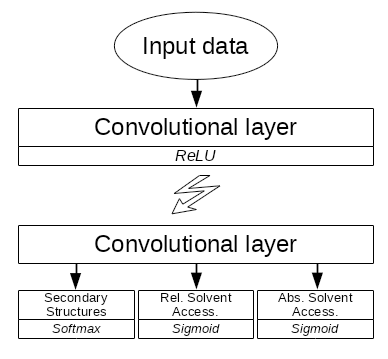
\includegraphics[width=\linewidth]{../graphs/arch}
 \captionsetup{width=0.8\linewidth, font=small}
 \captionof{figure}{Model architecture: The lightning represents one or more similar convolutional layers.}
\end{Figure}

\subsubsection{Training}
Utilizing the PyTorch loss function, autogradient and optimizer-libraries, implementing a model with essentially three losses is easy. As mentioned above, the model had a Cross Entropy loss for the secondary structure prediction, as well as two Binary Cross Entropy losses for the two solvency features. Training the model with regards to minimizing these losses is acheived simply by letting a variable be the sum of the three, and then letting the library automatically backtrace each of the parameters in the model via this value.
\begin{lstlisting}
# Calculate losses
loss1 = loss_func_structure(calc_struct,  correct_struct)
loss2 = loss_func_solvent(calc_rel, correct_rel)
loss3 = loss_func_solvent(calc_abs,  correct_abs)

# Sum the losses
loss_sum = (loss1 + loss2 + loss3)

# Backpropagate and train
loss_sum.backward()
optimizer.step()
\end{lstlisting}


\subsubsection{Accuracy}
Evaluating the accuracy of the model's predictions happens for each of the three features being predicted in the model.\\
The accuracy of the secondary structure label prediction happens in a similar fashion to the one in the single-task model. Seing as we know the structure of the solvent accessibility features to be binary and independent (an amino acid can be relatively solvent while not absolutely solvent and vica-versa), we can, after manually applying a sigmoid function on them, employ a simple round function to convert the probability outputted by the model to a binary prediction.\\
Having done so, the same method of constructing a matrix of correct and false predictions and then filtering this matrix by the mask already derived from the secondary structures was used.


\subsection{Hyperparameters}
In order to optimize our two models we iterated over a series of values for the models' hyperparameters, that is the number of layers, the depth of the layers, the learning rate and the size of the kernels used in the convolutions.\\
For a starting point, we chose to adapt the values used by Xi et. al, and then iterated to both sides of those values.\\
An initial decision to make was the batch size - that is how many inputs from the data set to process at once. In general there are three approaches how many data points to train on at once, compared to the total length of the data (LOD):
\begin{center}
\begin{tabular}{l|c}
\hline 
Name & Size \\ 
\hline 
Batch gradient & Size = LOD \\ 

Minibatch gradient & 1 $<$ Size $<$ LOD \\ 

Generative Stochastic & 1 \\ 
\hline 
\end{tabular} 
\end{center}
In the case of Generative Stochastic networks, the model is continuously trained on random single data points, and is generally accepted to produce better predictions than both batch and mini-batch gradient descents, however at the cost of increased training time.
Batch gradient was not an option for us, for the simple practical reason that there was not enough memory on our GPU to handle the entire data set at once. We opted for a batch size of 4 throughout our tests in a compromise between predictive power and speed of training.
A test of accuracy over different batch sizes can be found in the appendix.










